\section{Overfitting and Regularized Logistic Regression}

\subsection{Part 1}
Plot the sigmoid function $\frac{1}{1 + e^{-uX}}$ vs. $X \in \mathbb{R}$ for increasing weight $u \in \{1, 5, 100\}$. A qualitative sketch is enough. Use these plots to argue why a solution with large weights can cause logistic regression to overfit.
\begin{qsolve}
	\begin{qsolve}[]
		\begin{figure}[H]
			\centering
			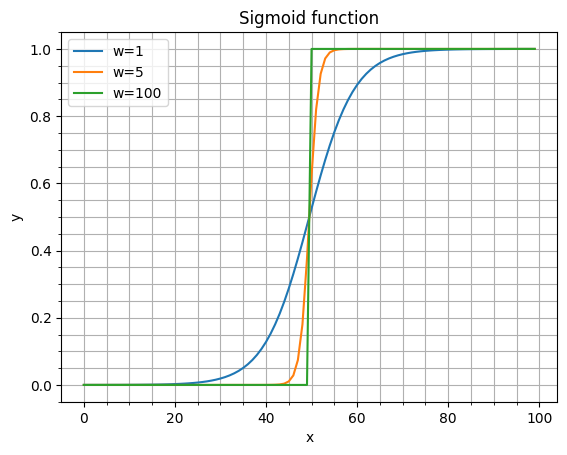
\includegraphics[width=0.7\textwidth]{sigmoid.png}
			\caption{Sigmoid function for increasing weight $w$}
		\end{figure}
		As the weight $w$ increases, the sigmoid function becomes steeper, which means that the output of the logistic regression model will be more sensitive to small changes in the input. This can cause the model to fit the training data too closely, capturing noise in the data rather than the underlying pattern. This is known as overfitting, and it can lead to poor generalization performance on new, unseen data.
	\end{qsolve}
\end{qsolve}
\subsection{Part 2}
To prevent overfitting, we want the weights to be small. To achieve this, instead of maximum conditional likelihood estimation (M(C)LE) for logistic regression:
\[
\max_{w_{0},\ldots,w_{d}} \prod_{i=1}^n P(Y_i \mid X_i, w_0, \ldots, w_d),
\]
we can consider maximum conditional a posteriori (M(C)AP) estimation:
\[
\max_{w_{0},\ldots,w_{d}} \left( \prod_{i=1}^n P(Y_i \mid X_i, w_0, \ldots, w_d) \right) P(w_0, \ldots, w_d)
\]
where $P(w_0, \ldots, w_d)$ is a prior on the weights. Assuming a standard Gaussian prior $N(0, I)$ for the weight vector, derive the gradient ascent update rules for the weights.
\begin{qsolve}
	\begin{qsolve}[]
		
		\[
		P(\omega \mid D) \propto P(\omega) P(D \mid \omega)
		\]

		\[
		P(\omega) = \frac{1}{(2\pi)^{\frac{d}{2}}} \exp\left(-\frac{1}{2} \omega^t I^{-1} \omega\right) = \frac{\exp(-\frac{1}{2} \omega^t I^{-1} \omega)}{(2\pi)^{\frac{d}{2}}}
		\]

		\[
		\omega = \begin{bmatrix} \omega_1 \\ \vdots \\ \omega_d \end{bmatrix}
		\]

		\[
		P(D \mid \omega) = \prod_{i=1}^n P(y_i \mid x_i; \omega)
		\]

		The log of the posterior is then:
		$$
		\hat{\omega} = \arg\max_{\omega} P(\omega \mid D) = \arg\max_{\omega} \left(\log(P(\omega \mid D))\right)
		$$
		$$
		 = \arg\max_{\omega} \left(\sum_{i=1}^n \log(P(y_i \mid x_i; \omega)) - \frac{d}{2} \omega^\top I^{-1} \omega \right)
		$$
		
		$$
		f(\omega) = \sum_{i=1}^n \log(P(y_i \mid x_i; \omega)) - \frac{d}{2} \omega^\top I^{-1} \omega
		$$
		To find the weights that maximize this posterior, we use gradient ascent. The gradient of the log-posterior is:
		
		$$
		\text{Gradient ascent:} \quad \omega_{i}^{(t+1)} = \omega_{i}^{(t)} + \eta \nabla f(\omega)
		$$
		
		\[
		\frac{\partial f}{\partial \omega_i} = -\omega_i + \sum_{i=1}^n \frac{1}{P(y_i \mid x_i; \omega)} \frac{\partial P(y_i \mid x_i; \omega)}{\partial \omega_i}
		\]

		\[
		\frac{\partial f}{\partial \omega_i} = -\omega_i + \sum_{i=1}^n x_i y_i \left(\frac{1}{1+e^{-\omega^\top x_i}}\right) - x_i \frac{e^{-\omega^\top x_i}}{(1+e^{-\omega^\top x_i})^2}
		\]
		
		\[
		P(y=1 \mid x_i; \omega) = \frac{1}{1+e^{-\omega^\top x_i}}
		\]

		\[
		\Rightarrow \frac{\partial P(y=1 \mid x_i;\omega)}{\partial \omega_j} = x_{ij} \frac{e^{-\omega^\top x_i}}{(1+e^{-\omega^\top x_i})^2} = x_{ij} \left(\frac{1}{1+e^{-\omega^\top x_i}}\right) \left(1 - \frac{1}{1+e^{-\omega^\top x_i}}\right)
		\]
		\splitqsolve[\splitqsolve]
		\[
		P(y=0 \mid x_i; \omega) = 	\frac{e^{-\omega^t x_i}}{1+e^{-\omega^t x_i}}
		\]

		\[
			\Rightarrow \frac{\partial P(y=0 \mid x_i;\omega)}{\partial \omega_j} = -x_{ij} \frac{e^{-\omega^t x_i}}{(1+e^{-\omega^t x_i})} + x_{ij} \left(\frac{e^{-\omega^t x_i}e^{-\omega^t x_i}}{(1+e^{-\omega^t x_i})^2}\right)
		\]
		
		\[
		\frac{\partial P(y=1 \mid x_i, \omega)}{\partial \omega_j} = x_{ij} P(y=1 \mid x_i, \omega) (1 - P(y=1 \mid x_i, \omega))
		\]

		\[
		\frac{\partial P(y_i = 0 \mid x_i, \omega)}{\partial \omega_j} = - x_{ij} P(y_i = 1 \mid x_i, \omega) P(y_i = 0 \mid x_i, \omega)
		\]

		\[
		\frac{\partial f}{\partial \omega_j} = -\omega_j + \sum_{i=1}^n x_{ij} (y_i - P(y=1 \mid x_i, \omega))
		\]

		\[
		\omega_j^{(t+1)} = \omega_j^{(t)} + \eta \left(-\omega_j^{(t)} + \sum_{i=1}^n x_{ij} (y_i - P(y=1 \mid x_i, \omega))\right)
		\]
		\begin{center}
			\hl{$\omega_j^{(t+1)} = \omega_j^{(t)} (1-\eta) + \eta \sum_{i=1}^n x_{ij} \left(y_i - \frac{1}{1+e^{-(\omega^{(t)})^\top x_i}}\right)$}		
		\end{center}
		
		\end{qsolve}
\end{qsolve}